% Main manuscript: annual debit rules under a common soft-thermal DC network model.
\documentclass[10pt,journal]{IEEEtran}
\usepackage[T1]{fontenc}
\usepackage[utf8]{inputenc}
\usepackage{amsmath,amssymb,amsthm,mathtools,bm}
\usepackage{booktabs,tabularx,array,graphicx,cite,xurl}
\usepackage{algorithmic}
\usepackage{tikz,pgfplots}
\pgfplotsset{compat=1.18}
\usetikzlibrary{arrows.meta,positioning}
\usepackage[hidelinks]{hyperref}
\interdisplaylinepenalty=2500
\emergencystretch=1em
\newtheorem{proposition}{Proposition}
\newtheorem{theorem}{Theorem}
\newtheorem{lemma}{Lemma}
\newtheorem{corollary}{Corollary}
\newcounter{procedure}
\newcommand{\R}{\mathbb R}
\newcommand{\one}{\mathbf 1}
\newcommand{\pos}[1]{\left[#1\right]_+}
\newcommand{\Mone}{\mathrm{M1}}
\newcommand{\Mtwo}{\mathrm{M2}}
\newcommand{\Mlp}{\mathrm{M1\text{-}LP}}
\newcommand{\Mthree}{\mathrm{M3}}
\newcommand{\F}{\mathcal F}
\newcommand{\dd}{\mathrm d}
\title{Annual Restriction Accounting for Non-Firm Transmission Access: Entitlement Geometry and Network Effects}
\author{Alban Kryeziu, Stuart X.~Zhu, Tolga Karabas, and Evrim Ursavas%
\thanks{The authors are with the Department of Operations, Faculty of Economics and Business, University of Groningen, 9747 AE Groningen, The Netherlands. Corresponding author: Alban Kryeziu (e-mail: a.kryeziu@rug.nl).}}
\hypersetup{pdftitle={Annual Restriction Accounting for Non-Firm Transmission Access: Entitlement Geometry and Network Effects},pdfauthor={Alban Kryeziu, Stuart X. Zhu, Tolga Karabas, Evrim Ursavas}}
\begin{document}
\maketitle
\begin{abstract}
Non-firm transmission access permits partial restrictions, but an annual allowance does not define how each action depletes the remaining right. This paper compares touched duration, request-normalized debit, proportional depth, and conservative premiums under one network model. A relaxed hybrid duration-depth formulation projects exactly onto request-normalized accounting. Independently reconstructed supporting-plane lower bounds and feasible depth witnesses support guarded numerical separations from every annual touched-duration schedule. In a Dutch 45-bus model with 114 directional positions, the 2029--2031 separations are 14.7\%--20.8\%; complete dual multipliers are retained, but the bounds are not interval certificates. In 48-hour rolling evaluations, proportional depth reduces integrated overload by 22.1\%--26.8\% while increasing capacity-normalized exposure by 38.4\%--40.6\%. A marginal-relief premium improves residuals by 13.7\%--15.9\% over a uniform premium, but ordinary depth remains better. Retrospective positionwise energy controls reveal avoidable residuals in the uniform rolling allocation without establishing a prospective advantage of differentiated contracts. Selected alternating-current checks retain substantial thermal violations. The results characterize entitlement-dependent action domains and network outcomes, rather than equivalent customer protection or secure dispatch.
\end{abstract}
\begin{IEEEkeywords}
Annual entitlement, congestion management, debit accounting, non-firm transmission access, optimization, rolling horizon.
\end{IEEEkeywords}

\section{Introduction}
\label{sec:intro}
\IEEEPARstart{A}{n} annual non-firm restriction limit is incomplete without an action-debit rule. A 5-MW and a 100-MW restriction of a 100-MW position, each lasting one hour, consume two touched hours but 1.05 full-depth-equivalent (FDE) hours. Network effects depend on location, time, and magnitude; contractual depletion depends on the debit rule. The latter therefore changes the feasible annual sequence of network actions.

Flexible-connection studies examine firm versus non-firm admission, curtailment risk, and capacity sharing \cite{AnayaPollitt2015,DzamarijaKeane2013,Sedzro2021,Bjarghov2024}. De Santi \emph{et al.} compare pro-rata and technically efficient curtailment with connection-queue and fairness consequences \cite{DeSanti2025}, while Hennig \emph{et al.} analyze advance-notice and restriction-risk trade-offs \cite{Hennig2024RiskRestriction}. Oren and Smith study discretionary annual interruptions \cite{OrenSmith1992}; priority-service design and monthly constrained direct load control also treat contractual scarcity \cite{ChaoWilson1990,Fattahi2024}. These contributions explain how eligible capacity is admitted, allocated, or scheduled under prescribed contract terms. They leave open how different charges for the \emph{same partial restriction} change annual feasible-action domains when the connection portfolio and network model are fixed.

Network-constrained flexibility and congestion-contract studies address deliverability, procurement, redispatch, and risk \cite{VanDerHolst2024Activation,VanDerHolst2025Synergies,VanDerHolst2026RiskAware}. Here the access portfolio, requests, balancing keys, contingency evaluator, and nominal allowances are fixed. Only the action-to-entitlement accounting map changes. Since a constant debit already permits network-optimized differentiation across buses and hours, it is the appropriate control for differentiated accounting. Equal debit-hour allowances need not give equal energy or interruption burden.

Dutch time-duration transport rights motivate the annual scale. The 2024 regulatory decision specifies an 85\% contracted-availability guarantee. The decision of 23 April 2026 establishes announcement at 07:00 and administration in clock-quarter intervals \cite{ACM2024ATR,ACM2026TDTR}. Contracted availability differs from implemented curtailment when a user requests less than its contracted capacity. We accordingly study a stylized ledger of \emph{material implemented restrictions}, not the statutory availability counter. The hourly deterministic scenarios do not reproduce quarter-hour settlement or forecast-vintage announcements. Kryeziu \emph{et al.} \cite{Kryeziu2026AccessRights} study calendar construction, admission/routing, and grid-intervention decisions. Here those calendars and connections are inputs: the unresolved downstream question is how implemented restriction depth consumes an annual balance.

The contribution has three parts. \emph{First}, we characterize duration, depth, and hybrid debits, prove the exact projection of the relaxed support model, and identify the request-to-capacity denominator as a source of differing action domains after integrality is removed. \emph{Second}, we combine feasible annual depth actions with reconstructed lower bounds for the duration relaxation. This gives a strict separation test against \emph{every} feasible annual touched-duration schedule without requiring its mixed-integer optimum. Hourly supporting planes implement the annual comparison without dropping monitored hours or contingencies. \emph{Third}, we construct a conservative relief-based debit premium, compare it with uniform-premium and ordinary-depth controls, and use positionwise exposure witnesses to distinguish observed rolling gains from what the accounting rule itself makes possible. The numerical study reports physical exposure and selected AC limitations alongside residual improvements. Detailed derivations and diagnostic identities are provided in the separate technical report \cite{Kryeziu2026Technical}.

\section{Common Physical Model and Annual Resource}
\label{sec:model}
Positions $n\in\mathcal N$ represent separate import and export rights. Intervals $t\in\mathcal T$ have duration $\Delta_t>0$ hours. Capacity $P_n>0$ and requested transport $v_{nt}\geq0$ are in MW. Binary contract-duration and restriction-eligibility masks satisfy $\chi_{nt}\leq\kappa_{nt}$. The admissible restriction is
\begin{equation}
0\leq x_{nt}\leq b_{nt}:=\chi_{nt}\min\{P_n,v_{nt}\},
\qquad z_{nt}:=x_{nt}/P_n.
\label{eq:box}
\end{equation}
A zero request fixes the action, but does not shorten contracted duration. Requested injections use $v$, not the clipped bound $b$.

Let $A$ map restrictions to balanced bus-injection changes. With fixed background $p_t^{\rm bg}$,
\begin{align}
\one^\top A&=0,\qquad \one^\top p_t^{\rm bg}=0,\notag\\
p_t^{\rm req}&=p_t^{\rm bg}-Av_t,\qquad p_t(x_t)=p_t^{\rm req}+Ax_t.
\label{eq:balance}
\end{align}
Each column of $A$ represents one signed reduction of a directional transaction and a fixed balancing counter-injection. For interpretation, a column can be written as $A_{\cdot n}=\sigma_n(\pi_n-\omega_n)$ when the source and balancing participation vectors $\pi_n,\omega_n$ are nonnegative and each sums to one. The sign $\sigma_n$ encodes direction. All evaluations use the same study-specific columns rather than co-optimized redispatch. The counter-injection keys are not co-optimized and their generator headroom is not enforced. The accounting comparisons are conditional on this fixed response matrix. For retained network state $c$, the affine direct-current (DC) flow is
\begin{equation}
f_t^c(x_t)=\mathsf H^cp_t(x_t)+h^c
=f_t^{c,\rm req}+G^cx_t,\qquad G^c=\mathsf H^cA.
\label{eq:flows}
\end{equation}
Fixed tap and phase-shift effects are retained in $\mathsf H^c,h^c$ \cite{Stott2009}. A state-element row $(r,c)$ has rating $F_r^c>0$ and soft thermal bounds
\begin{equation}
-F_r^c-s^-_{rtc}\leq f_{rt}^c(x_t)\leq F_r^c+s^+_{rtc},
\qquad s^\pm_{rtc}\geq0.
\label{eq:thermal}
\end{equation}
One restriction vector is evaluated in every retained state; there is no corrective post-contingency recourse. The thermal inequalities are soft and are penalized rather than enforced as security constraints.

The primary and secondary objectives are
\begin{align}
S(x)&=\sum_t\Delta_t\sum_{c,r}\pos{|f_{rt}^c(x_t)|-F_r^c},\label{eq:S}\\
E(x)&=\sum_n E_n(x),\qquad E_n(x)=\sum_t\Delta_tx_{nt}.
\label{eq:E}
\end{align}
For debit rule $M$, minimize $S$ over $\F^M$, then minimize $E$ over its primary-optimal set. Finite bounds and closed debit constraints give attainment. Zero action is feasible because all thermal rows admit slack. The numerical secondary problem uses
\begin{equation}
\begin{aligned}
S(x)&\leq C_S:=S_I+\varepsilon(S_I),\\
\varepsilon(s)&=10^{-6}+10^{-9}\max\{1,|s|\}.
\end{aligned}
\label{eq:cap}
\end{equation}
The cap is based on the selected Stage-I incumbent, while its reconstructed lower bound is recorded separately.

The unit MW$\cdot$h$\cdot$row-state indicates summation of exceedance across monitored rows and states, not unserved energy or welfare. Unit commitment, participant ramping, additional balancing limits, storage intertemporal physics, and AC constraints are not optimized. Thermal slacks ensure algebraic feasibility even when substantial physical overload remains.

On the uniform grid, the nominal allowance is
\begin{equation}
H_n=\Delta\left\lfloor\rho\sum_t\kappa_{nt}\right\rfloor.
\label{eq:H}
\end{equation}
The primary comparisons use the same stored $H$, masks, and position ordering. Physical exposure is
\begin{equation}
D_n^2(x)=\sum_t\Delta_tz_{nt}=E_n(x)/P_n.
\label{eq:FDE}
\end{equation}
Its sum is measured in FDE directional-position-hours, not unique system hours or customers. Equal $H$ under different rules does not imply equal physical protection.

\section{A Family of Debit Rules and Its Geometry}
\label{sec:family}
\subsection{Duration, depth, and their continuous connection}
Touched time (M1) has binary support $u_{nt}$ and links
\begin{align}
\ell_{nt}&=\min\{b_{nt},\max(1\text{ MW},0.01P_n)\},\notag\\
\ell_{nt}u_{nt}&\leq x_{nt}\leq b_{nt}u_{nt},\qquad
\sum_t\Delta_tu_{nt}\leq H_n.
\label{eq:M1}
\end{align}
This bounds hours with a material positive action, not the number of contiguous events. M2 instead imposes $D_n^2(x)\leq H_n$ and allows submaterial actions. The distinction therefore includes both the debit unit and small-action admissibility.

A hybrid contract $H_\alpha$ uses
\begin{equation}
D_n^{H_\alpha}(x,u)=\sum_t\Delta_t[\alpha u_{nt}+(1-\alpha)z_{nt}]
\leq H_n,\quad 0\leq\alpha\leq1.
\label{eq:hybrid}
\end{equation}
For $\alpha>0$, retain the binary links in \eqref{eq:M1}. At $\alpha=0$, remove the links and support variables to recover M2, including submaterial actions. At $\alpha=1$, recover M1. The continuous request-depth interpolation is
\begin{equation}
D_n^{R_\beta}(x)=\sum_{t:b_{nt}>0}\Delta_tx_{nt}
\left[\frac{1-\beta}{b_{nt}}+\frac{\beta}{P_n}\right]\leq H_n.
\label{eq:request}
\end{equation}
Here $0\leq\beta\leq1$, and zero-bound coordinates are fixed to zero.

\begin{proposition}[Projection and hybrid connection]
\label{prop:projection}
Suppose $0\leq\ell_{nt}\leq b_{nt}$. The projection of the relaxed hybrid links ($0\leq u\leq1$) is exactly $\F^{R_{1-\alpha}}$. Hence $R_0$ is M1-LP and $R_1$ is M2. The threshold $\ell_{nt}$ disappears entirely upon projection. With equal durations and integer $H_n/\Delta$, the isolated position factor of $R_0$ is the convex hull of the M1 action set.
\end{proposition}
\begin{IEEEproof}
At $b_{nt}>0$, the least relaxed activation is $u_{nt}=x_{nt}/b_{nt}$. It satisfies both links because $\ell_{nt}\leq b_{nt}$. Since the hybrid debit is nondecreasing in $u$, a lift exists precisely when substituting this activation satisfies \eqref{eq:hybrid}. The resulting coefficient is $\alpha/b_{nt}+(1-\alpha)/P_n$, which is \eqref{eq:request} with $\beta=1-\alpha$. At $b=0$ take $u=x=0$. For the hull claim, rescale $y_t=x_{nt}/b_{nt}$ on positive-bound coordinates. The polytope is $0\leq y\leq1$, $\sum_ty_t\leq K_n$ with integer $K_n$. A vertex cannot have two fractional coordinates on a tight sum, or any fractional coordinate on a slack sum. A single fractional coordinate cannot make an integer tight sum. Every vertex is therefore binary and lifts to an M1 action at zero or $b_{nt}$, proving the hull equality.
\end{IEEEproof}
The threshold disappears because $u=x/b$ is feasible in the relaxation even when $0<x<\ell$. The hull statement concerns isolated actions, not the minimum of a coupled convex objective. For $P=b_1=b_2=2$, $\ell_1=\ell_2=1$, $H=\Delta=1$, and $S(x)=\pos{1-x_1}+\pos{1-x_2}$, M1 has minimum one whereas $(1,1)$ is relaxed-feasible with value zero.

\begin{proposition}[Ordered contractual resources]
\label{prop:hierarchy}
Under the common physical model, increasing $\alpha$ shrinks the hybrid action set, and increasing $\beta$ enlarges the request-depth set. In particular,
\begin{gather}
\F^{\Mone}\subseteq\F^{H_\alpha}\subseteq\F^{\Mtwo},\qquad
\F^{\Mone}\subseteq\F^{\Mlp}\subseteq\F^{\Mtwo}.\label{eq:hierarchy}
\end{gather}
Exact primary minima are ordered in the reverse direction of set inclusion. Attained lexicographic pairs are ordered too, but secondary energies alone need not be.
\end{proposition}
\begin{IEEEproof}
On a supported action $z_{nt}\leq u_{nt}$, so raising $\alpha$ raises its debit. The endpoint convention at zero only enlarges the admissible set. For $R_\beta$, $1/b_{nt}\geq1/P_n$, so raising $\beta$ reduces debit. The M1 relaxation gives the second chain. A common physical intersection preserves inclusion. If primary minima tie, the minimizing sets remain nested and order the secondary minima. Otherwise the primary component determines the lexicographic comparison.
\end{IEEEproof}
The continuous debit difference is
\begin{equation}
D_n^{1L}(x)-D_n^2(x)=\sum_{t:b_{nt}>0}\Delta_tx_{nt}
\left(\frac1{b_{nt}}-\frac1{P_n}\right)\geq0.
\label{eq:wedge}
\end{equation}
It vanishes on full-request coordinates. A positive difference on one trajectory need not violate its budget, and strict inclusion is not automatic. If every positive $b_{nt}=P_n$, the two continuous domains coincide. Fig.~\ref{fig:geometry} illustrates why this difference persists after relaxing the binary support.

\begin{figure}[t]
\centering
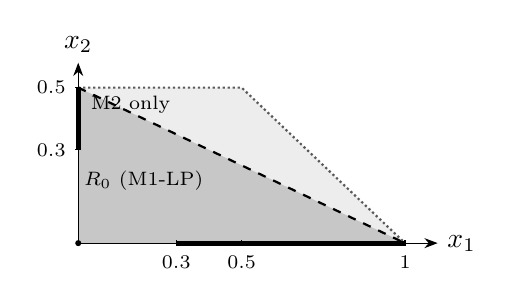
\begin{tikzpicture}[x=4.15cm,y=3.95cm,>=Stealth]
  \fill[black!7] (0,0)--(1,0)--(.5,.5)--(0,.5)--cycle;
  \fill[black!22] (0,0)--(1,0)--(0,.5)--cycle;
  \draw[black!65,densely dotted,thick] (0,.5)--(.5,.5)--(1,0);
  \draw[black,dashed,thick] (0,.5)--(1,0);
  \draw[->] (0,0)--(1.1,0) node[right] {$x_1$};
  \draw[->] (0,0)--(0,.58) node[above] {$x_2$};
  \foreach \x/\a in {.3/{0.3},.5/{0.5},1/{1}} {
    \draw (\x,.009)--(\x,-.009) node[below,font=\scriptsize] {$\a$};
  }
  \foreach \y/\a in {.3/{0.3},.5/{0.5}} {
    \draw (.009,\y)--(-.009,\y) node[left,font=\scriptsize] {$\a$};
  }
  \draw[black,line width=1.8pt] (.3,0)--(1,0);
  \draw[black,line width=1.8pt] (0,.3)--(0,.5);
  \fill (0,0) circle (1.1pt);
  \node[font=\scriptsize,align=center] at (.20,.20) {$R_0$ (M1-LP)};
  \node[font=\scriptsize,align=center] at (.16,.445) {M2 only};
\end{tikzpicture}
\caption{Two-hour action geometry ($P=1$, $b=(1,0.5)$, $\ell=(0.3,0.3)$, $H=\Delta=1$). M1 comprises the origin and heavy axial segments, $R_0$ the dark triangle, and M2 both shaded regions. The dashed and dotted boundaries give $x_1+2x_2=1$ and $x_1+x_2=1$.}
\label{fig:geometry}
\end{figure}

\subsection{State-weighted and depth-protective rules}
For a nonnegative, fixed rate schedule, define
\begin{equation}
D_n^q(x)=\sum_t\Delta_tq_{nt}z_{nt}\leq H_n.
\label{eq:weighted}
\end{equation}
M2 has $q=1$. A budget-dual baseline also permits discounts and surcharges. We denote the conservative rule with $q_{nt}\geq1$ by $C_q$ and the constant-premium control $q_{nt}=\bar q\geq1$ by $U_{\bar q}$. Then
\begin{equation}
\F^{C_q}(H)\subseteq\F^{\Mtwo}(H),\qquad
\F^{U_{\bar q}}(H)=\F^{\Mtwo}(H/\bar q).
\label{eq:conservative}
\end{equation}
The uniform premium tightens the physical allowance rather than changing the optimization algorithm. The equality uses $H/\bar q$, not a newly rounded allowance fraction in \eqref{eq:H}. Two premium domains need not be nested. With two unit-duration hours, $H=1$, unit normalized action bounds, $q=(1.5,1)$ and $\bar q=1.25$, $(z_1,z_2)=(0.8,0)$ satisfies only the uniform budget, whereas $(0,1)$ satisfies only the state-aware budget.

An additional depth-protection family is
\begin{equation}
D_n^{P_{\kappa,\tau}}(x)=\sum_t\Delta_t
[z_{nt}+\kappa\pos{z_{nt}-\tau}]\leq H_n,
\label{eq:progressive}
\end{equation}
with $\kappa\geq0$ and $0<\tau<1$. Nonnegative auxiliaries $h_{nt}\geq z_{nt}-\tau$ give an exact linear-programming (LP) representation. Its debit dominates physical FDE, so its action domain is contained in M2. This rule protects against deep restrictions rather than promising a lower annual residual. We retain it as a mathematical and fixed-policy diagnostic, not an optimized Dutch policy.

The full-depth normalization has a mathematical limit. If $g(0)=0$, $g(1)=1$, and $g$ is convex, then $g(z)\leq z$ on $[0,1]$. A convex depth surcharge cannot both dominate linear FDE at all depths and preserve those endpoints unless it equals FDE. In \eqref{eq:progressive}, full-depth debit is deliberately $1+\kappa(1-\tau)$.

\begin{corollary}[Limit of exposure-preserving design]
\label{cor:limit}
Any rule whose feasible actions satisfy $D_n^2(x)\leq H_n$ for every $n$, with the same physical model, obeys
\begin{equation}
S^{\Mtwo,*}(H)\leq S^{M,*}(H).
\label{eq:dominance}
\end{equation}
\end{corollary}
\begin{IEEEproof}
Its action domain is a subset of $\F^{\Mtwo}(H)$.
\end{IEEEproof}
Thus no conservative premium can improve on the global annual M2 minimum for the same $H$ and physical model. This is not a dominance result between rolling controllers: finite look-ahead and chronology can produce different suboptimal trajectories.

\begin{theorem}[Annual separation without an M1 optimum]
\label{thm:separation}
Let $L^{1L}\leq S^{\Mlp,*}$ be a valid lower bound. Let $x^c\in\F^{\Mtwo}$ and $S(x^c)\leq U^2$. If $U^2+\delta<L^{1L}$ with $\delta\geq0$, then $S(x^c)<S(x^1)$ for every $x^1\in\F^{\Mone}$. If $L^{1L}>0$, the relative reduction is at least $1-(U^2+\delta)/L^{1L}$.
\end{theorem}
\begin{IEEEproof}
The inclusions give
$S(x^c)\leq U^2\leq U^2+\delta<L^{1L}\leq S^{\Mlp,*}\leq S(x^1)$.
Divide by $S(x^1)\geq L^{1L}>0$ for the relative statement.
\end{IEEEproof}
The theorem is exact, conditional on valid endpoints. Section~\ref{sec:solution} distinguishes this statement from its guarded floating-point evaluation.

\section{Constructing State-Dependent Debit Premiums}
\label{sec:design}
\subsection{A limitation of budget-dual attribution}
The earlier three-bucket M3 baseline uses the Stage-II entitlement multiplier $\mu_{ny}$ and a selected M2 exposure $w_{nty}=\Delta_t x^{II}_{nty}/P_n$ to form $a_{nty}=\mu_{ny}w_{nty}$. Under regularity, this is a \emph{fixed-primary-cap} sensitivity of secondary energy, not the marginal change in primary overload or the derivative of the complete two-stage value when its primary cap changes with $q$ \cite{BonnansShapiro2000}. Bucket ratios $A_b/W_b$ average position-year multipliers and need not capture hourly network relief. The selected $\rho=0.15$ ridge-import aggregates satisfy a sufficient monotonicity condition for a flat ordered, mean-one card. Export uses a sparse-reference fallback; a nonuniform histogram candidate failed validation. Both adopted cards have $q=1$. Their original fitting problem and flatness proof appear in the companion.

\subsection{A score aligned with the network residual}
The alternative uses the primary network objective directly rather than a multiplier from the secondary energy objective. Let
$\psi_t(x_t)=\sum_{c,r}\pos{|f_{rt}^{c,\rm req}+G^c_{r\cdot}x_t|-F_r^c}$.
For $b_{nt}>0$, define the right directional relief per FDE hour by
\begin{equation}
m_{nt}=-P_n\psi_t'(0;e_n).
\label{eq:score}
\end{equation}
In the following expression, $j$ indexes every retained state-element row, $f_{jt}=f_{jt}^{\rm req}$, and $G_{jn}$ is its restriction sensitivity:
\begin{align}
m_{nt}=-P_n\bigg[&\sum_{j:f_{jt}>F_j}G_{jn}-\sum_{j:f_{jt}<-F_j}G_{jn}\notag\\
&+\sum_{j:f_{jt}=F_j}\pos{G_{jn}}
+\sum_{j:f_{jt}=-F_j}\pos{-G_{jn}}\bigg].
\label{eq:scoreexplicit}
\end{align}
The boundary terms include newly induced overload. Duration cancels when hourly residual change is divided by $\Delta_tx_{nt}/P_n$. The score has units of integrated residual per FDE hour, summed over rows rather than averaged. A positive score means infinitesimal relief at the unrestricted-request state. Signed sensitivities and later hinge changes prevent interpreting it as a global independent ranking of joint actions.

All 8,837 rows enter the derivative. Zero-bound coordinates have no fitting exposure; a finite-step probe can cross a hinge and differ from this local score.

\subsection{A conservative ordered premium card}
The reference weights are the M2 fitting-year exposures $w_{nty}=\Delta_tx_{nty}^{II}/P_n$, without dual multipliers. Import and export observations are pooled. Exposure-weighted score tertiles define buckets $\mathcal B_1,\mathcal B_2,\mathcal B_3$, from low to high relief. Thresholds and tie assignments are learned only from fitting data and fixed in subsequent years. Put
\begin{equation}
W_b=\sum_{(n,t,y)\in\mathcal B_b}w_{nty},\qquad
\bar m_b=\frac{\sum_{(n,t,y)\in\mathcal B_b}w_{nty}m_{nty}}{W_b}.
\label{eq:bucket}
\end{equation}
All three executed buckets have positive weight. Let $s=\max\{1,\max_b|\bar m_b|\}$ in the reported score units and $\widetilde m_b=\bar m_b/s$. For a prescribed reference mean $\bar q=1+\xi$ and upper premium $1+\gamma$, solve
\begin{align}
\min_q\quad&\sum_bW_b\widetilde m_bq_b+
\frac{\lambda}{2}\sum_bW_b(q_b-\bar q)^2,\notag\\
\text{s.t.}\quad&q_1\geq q_2\geq q_3,\quad1\leq q_b\leq1+\gamma,\notag\\
&W^\top q=\bar qW^\top\one.
\label{eq:newcard}
\end{align}
Higher-benefit buckets receive no higher debit. The quadratic term limits departures from the uniform premium. This is a rate-design surrogate, not a derivative of annual rolling performance with respect to the complete card.

\begin{proposition}[Card existence and differentiation]
\label{prop:card}
For $0\leq\xi\leq\gamma$, the feasible set of \eqref{eq:newcard} is nonempty and compact. If all $W_b>0$ and $\lambda>0$, its minimizer is unique. If also $0<\xi<\gamma$, $\bar m_1\leq\bar m_2\leq\bar m_3$, and $\bar m_1<\bar m_3$, that minimizer is nonuniform.
\end{proposition}
\begin{IEEEproof}
The constant vector $\bar q\one$ is feasible. Positive diagonal quadratic weights give strict convexity. At that constant vector the quadratic gradient vanishes. The feasible direction $d=(1/W_1,0,-1/W_3)$ preserves the mean and ordering for a sufficiently small positive step within the bounds. Its linear derivative is $\widetilde m_1-\widetilde m_3<0$. The constant card therefore cannot minimize the objective.
\end{IEEEproof}
If $q\geq1$ were combined with a mean-one constraint, every positive-weight bucket would instead be forced to one. The positive mean premium is therefore explicit. It is a chosen contract-design scenario, not an estimate of customer disutility or a regulatory requirement. A uniform card with the same mean is the necessary control.

For $\gamma=0.5$, $\xi=0.25$, and $\lambda=1$, fitted thresholds 123.899047 and 570.721461 and score scale $s=3895.515232$ give
\begin{equation}
q^C=(1.4073554014,\ 1.3426166214,\ 1),\quad q^U=1.25.
\label{eq:rates}
\end{equation}
The uniform control matches pooled fitting exposure, not directional means (1.226928 import, 1.319258 export) or realized exposure (Fig.~\ref{fig:ratecard}); the latter is tested separately.

\begin{figure}[t]
\centering
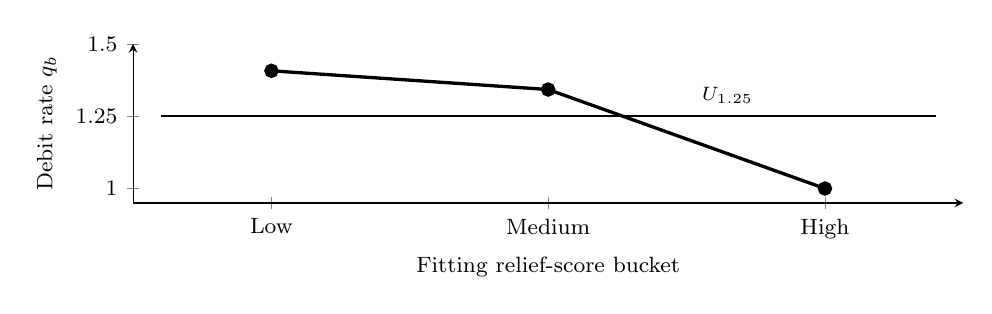
\begin{tikzpicture}
\begin{axis}[width=\columnwidth,height=3.6cm,ymin=0.95,ymax=1.5,
 xmin=0.5,xmax=3.5,xtick={1,2,3},xticklabels={Low,Medium,High},
 xlabel={Fitting relief-score bucket},ylabel={Debit rate $q_b$},
 ytick={1,1.25,1.5},tick label style={font=\footnotesize},
 label style={font=\footnotesize},axis lines=left,clip=false]
\addplot[black,thick] coordinates {(0.6,1.25) (3.4,1.25)};
\addplot[black,very thick,mark=*,mark size=2pt] coordinates {(1,1.4073554014) (2,1.3426166214) (3,1)};
\node[anchor=south west,font=\scriptsize] at (axis cs:2.52,1.26) {$U_{1.25}$};
\end{axis}
\end{tikzpicture}
\caption{Frozen conservative premium by increasing relief-score bucket. The uniform control matches the pooled fitting-exposure mean, not each position's realized exposure.}
\label{fig:ratecard}
\end{figure}




\subsection{Chronological use and exposure-controlled witnesses}
At epoch $k$, a 48-hour window $\mathcal L_k$ is optimized under remaining balance $B_{nk}$. Only its first 24 hours $\mathcal I_k$ are implemented:
\begin{align}
\sum_{t\in\mathcal L_k}\Delta_td^M_{nt}&\leq B_{nk},\notag\\
B_{n,k+1}&=B_{nk}-\sum_{t\in\mathcal I_k}\Delta_td^M_{nt},\quad B_{n0}=H_n,
\label{eq:rolling}
\end{align}
where $d^M=u$ for M1, $z$ for M2, and $qz$ for weighted rules. The final window is truncated, implemented blocks partition the year, and unimplemented overlaps are reconsidered. There is no terminal reserve or continuation value. In exact arithmetic nonnegative implemented debit and the window constraint preserve nonnegative balances, so telescoping proves annual feasibility.

The executed $C_q$ has one weighted ledger. A second physical ledger is redundant when all $q\geq1$: past weighted debit dominates past FDE, and any future physical debit is bounded by its weighted debit. This argument fails under discounts. We do not describe the experiment as a discount-capable two-ledger policy. In the reported rolling experiment, the 48-hour injection and request trajectories and the score used to assign each rate are evaluated on the same deterministic scenario realization. The resulting controller is an information-rich retrospective benchmark. It is not a nonanticipative simulation of announcements at 07:00. To administer such a rule prospectively, $q_{nt}$ and the restriction schedule for an announced period must be measurable with respect to information available at its announcement time and frozen thereafter. Replacing $f_t^{\rm req}$ by its timestamped forecast $\widehat f_{t\mid\tau}^{\rm req}$ in \eqref{eq:score} is a possible construction, but no matching forecast-vintage experiment has been run. The current 24-hour implementation blocks also do not reproduce legal quarter-hour settlement.

Let $x^C$ and $x^U$ be separately guarded annual witnesses. Define $x^{EC}_{nt}=\alpha_nx^C_{nt}$ using
\begin{equation}
\alpha_n=\begin{cases}
\min\{1,E_n(x^U)/E_n(x^C)\},&E_n(x^C)>0,\\
1,&E_n(x^C)=0,
\end{cases}
\label{eq:energywitness}
\end{equation}
Conservative numerical factors are used in the implementation.

\begin{proposition}[A common-feasible exposure witness]
\label{prop:energywitness}
For fixed nonnegative rates and the present soft-thermal model, $x^{EC}\in\F^{C_q}\cap\F^{U_{\bar q}}$ and $E_n(x^{EC})\leq E_n(x^U)$ for every position.
\end{proposition}
\begin{IEEEproof}
The box is preserved by contraction. Each weighted $C_q$ debit weakly decreases. The energy inequality follows from \eqref{eq:energywitness}, and
$D_n^{U_{\bar q}}(x^{EC})=\bar q E_n(x^{EC})/P_n\leq\bar q E_n(x^U)/P_n\leq H_n$.
Thermal slack preserves model feasibility.
\end{IEEEproof}
The witness therefore also belongs to the uniform control's annual action domain. If it improves on the recorded uniform rolling action, it demonstrates an avoidable residual in that action, not the impossibility of attaining the same outcome under uniform accounting. Its construction uses completed annual trajectories. It is not the output of a prospective energy-matched rolling controller. Prefix-budget feasibility alone does not establish such a controller claim.

\section{Annual Solution and Numerical Verification}
\label{sec:solution}
\subsection{Safe screening and an hourly support master}
The annual debit couples otherwise separable hourly network evaluations. Write
\begin{equation}
\phi_t(x_t)=\Delta_t\psi_t(x_t)=\sum_{j\in\mathcal J_t}\pos{a_{tj}^\top x_t+b_{tj}},
\label{eq:hinges}
\end{equation}
so $S(x)=\sum_t\phi_t(x_t)$. For each monitored state-element row $j=(r,c)$, the two hinge pairs are $(a,b)=(\Delta_tG^c_{r\cdot},\Delta_t(f_{rt}^{c,\rm req}-F_r^c))$ and $(a,b)=(-\Delta_tG^c_{r\cdot},\Delta_t(-f_{rt}^{c,\rm req}-F_r^c))$. Thus $a_{tjn}\geq0$ means that increasing restriction $x_{nt}$ cannot relieve that signed candidate exceedance. Positive ratings ensure that both directed exceedances cannot be active simultaneously.

\begin{proposition}[Safe reduction for monotone debit]
\label{prop:screen}
A hinge can be removed if
\begin{equation}
\overline d_{tj}=b_{tj}+\sum_n\max\{0,a_{tjn}b_{nt}\}\leq0.
\label{eq:screen}
\end{equation}
If $a_{tjn}\geq0$ for each potentially positive hinge at a coordinate $(n,t)$, fixing $x_{nt}=0$ preserves the optimal objective pair, provided debit cannot increase under that reduction and no other constraint requires positive action.
\end{proposition}
\begin{IEEEproof}
Equation~\eqref{eq:screen} is the affine maximum over the full box. For a retained hinge with nonnegative coefficient, decreasing the coordinate cannot raise its value. Energy and monotone debit also do not increase. In the supported rules, set the corresponding $u$ to zero. Applying this transformation to an optimum proves value preservation.
\end{IEEEproof}
The hypotheses hold for the executed positive-weight rules. Unchanged physical bounds alone would not justify action elimination for a temporally coupled debit. Fixed-action hours contribute a constant $C_0$, and every original row and timestamp remains in final replay.

For $J\subseteq\mathcal J_t$, define $\ell_{tJ}(x_t)=\sum_{j\in J}(a_{tj}^\top x_t+b_{tj})$. Then
\begin{equation}
\phi_t(x_t)=\max_{J\subseteq\mathcal J_t}\ell_{tJ}(x_t).
\label{eq:support}
\end{equation}
Every partial sum is a minorant. The set of strictly positive terms attains equality at its anchor. With one epigraph variable $\theta_t\geq0$ per retained hour, the master imposes stored supports $\theta_t\geq\ell_{tJ}(x_t)$. Its objective is $C_0+\sum_{t\in\mathcal T_{\rm ret}}\theta_t$, with fixed-hour residuals in $C_0$ exactly once. Full replay supplies violated tight supports. This is an hourly disaggregated supporting-plane construction \cite{Kelley1960,BirgeLouveaux1988}. Every retained hour and contingency remains in the evaluation.

For a continuous rule $M\in\{\Mlp,\Mtwo,U_{1.25},C_q\}$, let $\mathcal L_k^r$ denote retained hours in window $\mathcal L_k$. Its restricted master is
\begin{equation}
\begin{aligned}
\mathcal M_k(\mathcal C):=\{(x,\theta):\ &x\in\mathcal X_k^M(B_k),\\
&\theta_t\geq 0,\ \theta_t\geq\ell_{tJ}(x_t),\ J\in\mathcal C_t,\ t\in\mathcal L_k^r\},\\
\widehat S_k(\theta)&=C_{0,k}+\sum_{t\in\mathcal L_k^r}\theta_t.
\end{aligned}
\label{eq:masterfamily}
\end{equation}
Here $\mathcal X_k^M(B_k)$ contains the physical bounds and the continuous debit ledger, $J_t(x_t)=\{j:a_{tj}^{\top}x_t+b_{tj}>0\}$, and $E_k(x)=\sum_{n,t\in\mathcal L_k}\Delta_tx_{nt}$. Algorithm~\ref{alg:solve} describes the implemented continuous-policy support route. The historical M1 windows instead use a guarded explicit-row mixed-integer formulation, with the same physical objective and chronological debit update.
\begin{figure}[b]
\centering
\begin{minipage}{0.98\columnwidth}
\footnotesize\hrule\smallskip
\refstepcounter{procedure}\label{alg:solve}
\textbf{Algorithm \theprocedure. Continuous-policy hourly supports and debit}\par
\begin{algorithmic}[1]
\STATE \textbf{Input:} Continuous $M$, $B_{n0}=H_n$, $(\mathcal L_k,\mathcal I_k)_{k=0}^{K-1}$.
\FOR{$k=0,\ldots,K-1$}
\STATE Screen \eqref{eq:screen}; seed $\mathcal C_t$ with $J_t(0)$ and validated selector hints.
\FOR{$r\in\{I,II\}$}
\REPEAT
\IF{$r=I$}
\STATE $(x,\theta)\in\arg\min_{\mathcal M_k(\mathcal C)}\widehat S_k(\theta)$.
\ELSE
\STATE $(x,\theta)\in\arg\min_{\substack{\mathcal M_k(\mathcal C)\\\widehat S_k(\theta)\leq C_{S,k}}}E_k(x)$.
\ENDIF
\STATE Replay $S(x)$ and hourly gaps $g_t=\phi_t(x_t)-\theta_t$.
\STATE If the stage test below fails, add tight selectors at underestimated hours.
\UNTIL{Stage I: aggregate and maximum positive gaps are within $\tau_f$; Stage II: replayed $S(x)\leq C_{S,k}+\tau_f$.}
\IF{$r=I$}
\STATE $S_{I,k}\gets C_{0,k}+\sum_{t\in\mathcal L_k^r}\phi_t(x_t)$; $C_{S,k}\gets S_{I,k}+\varepsilon(S_{I,k})$.
\ENDIF
\ENDFOR
\STATE $x_t^{\rm roll}\gets x_t$, $t\in\mathcal I_k$; $B_{n,k+1}\gets B_{nk}-\sum_{t\in\mathcal I_k}\Delta_td^M_{nt}(x)$.
\ENDFOR
\STATE Repair, replay, and verify physical and debit constraints.
\end{algorithmic}
\smallskip\hrule
\end{minipage}
\end{figure}
Here $\tau_f$ is the recorded numerical face tolerance; complete-row replay is also required. In exact arithmetic use $\tau_f=0$. Each unsuccessful solve adds a tight support, giving finite termination without a polynomial bound. Stage II need not make every epigraph tight once its replayed action meets the primary cap. The M1 mixed-integer engine uses explicit physical rows and a separate numerical face guard; its saved runs must not be described as hourly-master executions. Stage~II minimizes energy on the $\varepsilon$-capped primary level, not the exact lexicographic optimum. For floating-point solves, the master acceptance test uses stated tolerances, and the implemented trajectory is kept separate from the repaired annual witness.

\subsection{Dual reconstruction and feasible witnesses}
Let $Dx\leq H$ contain the linear debit rows after screening, $0\leq x\leq\bar x$, and $a_{tk}^\top x+b_{tk}\leq\theta_t$ the stored supports. Choose $\lambda,\zeta\geq0$ with $\sum_k\zeta_{tk}\leq1$, and put $r_I=D^\top\lambda+\sum_{t,k}\zeta_{tk}a_{tk}$. A valid Stage-I lower bound is
\begin{equation}
L_I=C_0-H^\top\lambda+\sum_{t,k}\zeta_{tk}b_{tk}
+\sum_j\bar x_j\min\{r_{I,j},0\}.
\label{eq:lowerI}
\end{equation}
Indeed, adding the nonnegative-multiplier constraint terms to the objective gives a Lagrangian minorant. Its infimum over $\theta\geq0$ is finite under the multiplier-sum condition. Minimizing the remaining linear function over the box gives the final correction. This term cannot be dropped when stationarity has a residual.

For Stage II, let $e$ contain the coefficients of $E$, and $\eta\geq0$ multiply its primary cap. With $\sum_k\zeta_{tk}\leq\eta$ and $r_{II}=e+D^\top\lambda+\sum_{t,k}\zeta_{tk}a_{tk}$, the same argument gives
\begin{align}
L_{II}={}&-H^\top\lambda+\sum_{t,k}\zeta_{tk}b_{tk}
+\eta(C_0-C_S)\notag\\
&+\sum_j\bar x_j\min\{r_{II,j},0\}.
\label{eq:lowerII}
\end{align}
These are analytical bounds for any admissible multipliers. The historical archive lacks complete dual vectors. A separate verification now reconstructs all three annual M1-LP masters from archived selectors on the complete physical box, with all hourly epigraphs and $C_0=0$. It retains raw and sign/sum-corrected multipliers, checks hourly sums by exact rational arithmetic, and evaluates \eqref{eq:lowerI} through support-column and physical-row paths. Coefficient-formation, accumulation, and scalar-reduction estimates give downward guards of $9.42\times10^{-5}$, $2.93\times10^{-5}$, and $9.68\times10^{-6}$ residual units. These are guarded floating-point bounds, not fully outward-rounded interval certificates.

After any required box projection of a nonnegative candidate, let $d_n$ be its actual linear debit. A separate witness scales each position by $0\leq\alpha_n\leq\min\{1,H_n/d_n\}$ when $d_n>0$. Set $\alpha_n=0$ if $H_n=0<d_n$ and retain a zero-debit action. A downward numerical guard is followed by independent checks. Full thermal replay is required because reducing a helpful restriction can raise $S$. In particular,
\begin{equation}
|S(x')-S(x)|\leq\sum_{t,c,r,n}\Delta_t|G_{rn}^c|\,|x'_{nt}-x_{nt}|.
\label{eq:lipschitz}
\end{equation}
The bound follows from the one-Lipschitz absolute value and positive part. Witness evaluation uses replay rather than substituting this potentially loose estimate.

The annual comparison uses
\begin{equation}
\delta=\max\{10^{-6},10^{-9}\max(1,|U^2|,|L^{1L}|)\}.
\label{eq:delta}
\end{equation}
This margin does not establish endpoint validity. The new lower bounds use the independently retained multipliers. The original B03 M2 witnesses pass exact stored-coordinate box and annual-debit checks, and independent full-row replay. Replay-error estimates are below $0.0061$ residual units; subtracting them additionally leaves all separation margins positive. No fully interval-certified separation is claimed. Raw rolling M1 actions have small documented link and box residuals and are not used as exact upper endpoints. None is needed for Theorem~\ref{thm:separation}.

\section{Dutch Case and Experimental Protocol}
\label{sec:case}
\subsection{Common data and boundaries}
The public-data Dutch model \cite{Zomerdijk2022,ZomerdijkData} has a 383-bus structural layer (730 lines and 33 transformers) used for localization and sensitivity comparison. All policy optimization uses the 45-bus 220/380-kV layer (92 lines and three transformers). The intact state and 93 retained non-islanding single-element outages produce
\begin{equation}
95+93(95-1)=8{,}837
\label{eq:rowcount}
\end{equation}
state-element rows per hour, with the outaged element omitted from its own state. Unsupported and islanding outages are excluded, so this is a declared contingency set rather than exhaustive Dutch $N-1$ security.

There are 114 directional positions (79 direct, 35 multibus). Multibus admission compares sensitivity errors with direct positions over 88 interfaces and 87 aligned states. The cutoffs are 2.135 for relative $\ell_2$ error, 5.212 for relative maximum error, 0.80 for material-sign agreement, and 0.40 for top-10 overlap. The first two allow 213.5\% and 521.2\% normalized error; small reference sensitivities can inflate these ratios, but no critical-line absolute-error bound follows. Sign and overlap filters measure direction and ranking, not electrical equivalence. The 45-bus layer is therefore a controlled DC testbed.

Provincial demand, photovoltaic, onshore-wind, and offshore-wind series are mapped separately by nonnegative, column-normalized weights. Future profiles reuse historical 2017 (non-leap) and 2016 (leap) shapes, scaled to constructed energy trajectories. Participant nominations are deterministic technology/day/hour profiles, \emph{not observed customer requests}. Fixed interchange, bounded background generation, and renewable downward adjustments are resolved before restriction optimization; background renewable reductions do not consume customer debit. The 24 registered immediate inputs are hash-identifiable, while some upstream public-release and generator-revision bindings remain unverified.

The chronology contains 61,344 UTC hours from 2025 to 2031, including leap-year 2028. The constructed nominations contain 6,993,216 position-hour values for the 114 directional positions. Positive-allowance positions number 3, 7, 41, 59, 72, 83, and 93 by year. Thus at least 291 of 342 fitting position-years have zero M2 allowance and zero exposure attribution. The scenarios are not observations of future Dutch operation. Averaging preserves linear physical debit but not touched duration: one restricted quarter-hour consumes 0.25 touched hours, whereas its positive hourly average may touch a whole hour.

\subsection{Calibration, evaluation, and information}
The duration/depth comparisons use $\rho=0.15$. Annual M1-LP and M2 are solved on each evaluation year; rolling M1 and M2 use the same 48-hour information horizon and 24-hour implemented block. A secondary premium-sensitivity exercise also used $\rho=0.03$. The budget-dual three-bucket baseline was fitted on 2025--2027 and selected on 2028; both selected cards were flat. Nonuniform candidates that failed the 2028 selection criterion were not evaluated as adopted policies.

The relief-based $C_q$ uses $\rho=0.15$, score scaling, pooled fitting weights, $\gamma=0.5$, $\xi=0.25$, and $\lambda=1$. These settings and a 0.1\% improvement gate against $U_{1.25}$ were fixed before optimization of the new policy trajectories. The card satisfies the 2028 gate and is held fixed for 2029--2030 and the 2031 confirmation. The premium design follows the first duration/depth analysis. Its fixed 2029--2031 assessments are temporally held out from fitting and validation, but are not untouched tests of the full research design process. The premium comparison consists of eight computed rolling trajectories (two policies in 2028--2031) under identical network inputs and solver settings.

The duration-matched diagnostic reoptimizes rolling M2 with position budgets $\widehat H_n=E_n(x^{1,\rm roll})/P_n$ obtained after the completed M1 year. The premium diagnostic instead contracts the completed $C_q$ trajectory using \eqref{eq:energywitness}. Both use hindsight exposure and are explicitly retrospective. Request-based interpolation $R_{0.5}$ and progressive debit with $(\kappa,\tau)=(1,0.5)$ are evaluated only on fixed actions. Their optimized policies were not computed.


\subsection{Replay and selected nonlinear checks}
Six hours per evaluation year were selected before AC outcomes: two for unrestricted-request stress, two for rolling M1/M2 discrepancy, and two for annual M2/M3 discrepancy. Deterministic deduplication and fill retain 18 hours. Flat M3 makes the last criterion tied (the predetermined tie-break selects the earliest UTC hours). Each hour includes the intact state and two selected outages. Thirteen reference and policy variants give 702 cases. Independent DC reconstruction uses the same injections and electrical data through a separate equation path, with row tolerance $\max\{10^{-4}\text{ MW},10^{-8}F_r\}$ and material-flow threshold $10^{-6}$ MW.

AC power flow in pandapower \cite{Thurner2018} retains the source reactive injections, generator dispatch, voltage controls, reactive limits, taps, shunts, and connection weights. The slack supplies losses. Unity, 0.98 lagging, and 0.98 leading participant power factors give 2,106 records. Thermal loading is the native current-based line measure and configured transformer measure \cite{PandapowerLoading,PandapowerTransformer}. The ordering indices are
\begin{align}
J^{DC}&=\sum_e\pos{|P_e^{DC}|/F_e-1},\notag\\
J^{AC}&=\sum_e\pos{\lambda_e^{AC}-1}.
\label{eq:J}
\end{align}
Here $\lambda_e^{AC}$ is loading percent divided by 100. A policy-difference deadband of $10^{-4}$ separates ties from material orderings. This normalized comparison is not the annual unnormalized objective $S$. The $C_q$ and $U_{1.25}$ trajectories, and their later exposure-capped witnesses, were not included in these AC runs. Consequently no AC feasibility rate can be inferred for them from this registry.

\section{Results}
\label{sec:results}
\subsection{Annual accounting separation}
The principal annual finding concerns \emph{action domains}, not a comparison of two incumbents. The independently reconstructed guarded M1-LP lower bound exceeds the original feasible M2 witness in each year (Table~\ref{tab:certificate}). Complete new multipliers and both certificate calculations are retained; the separation remains qualified by finite-precision arithmetic. Because M1-LP already relaxes the support binaries and materiality floor, the gap cannot be attributed solely to mixed-integer suboptimality. The distinct request- and capacity-based denominators in \eqref{eq:wedge} remain after that relaxation.

\begin{table*}[t]
\centering
\caption{Independent guarded M1-LP lower bounds and original feasible M2 witnesses at $\rho=0.15$ (millions of MW$\cdot$h$\cdot$row-state). Displayed lower/upper endpoints are rounded downward/upward. Margins and percentages use full-precision records. Complete new duals are retained; the arithmetic is not interval-certified.}
\label{tab:certificate}
\footnotesize
\begin{tabular}{@{}crrrrr@{}}
\toprule
Year & Selected M2 replay & Guarded M2 $U^2$ & M1-LP lower $L^{1L}$ & Separation margin & Relative bound (\%)\\
\midrule
2029 & 48.058421884 & 48.058421891 & 57.909827749 & 9.851406 & 17.0\\
2030 & 32.237842047 & 32.237842053 & 37.782287250 & 5.544445 & 14.7\\
2031 & 18.740819464 & 18.740819468 & 23.658821383 & 4.918002 & 20.8\\
\bottomrule
\end{tabular}
\end{table*}

Witness repair raises $S$ by only about 0.0065, 0.0050, and 0.0035 full units. Its logical role is feasibility, not a material change in the reported separation. The new lower endpoints differ from the historical scalars by less than 0.003 residual units; the displayed percentage conclusions are unchanged. Their qualification concerns guarded arithmetic rather than missing new dual vectors.

On the annual M2 actions, the projected-minus-depth debit totals are 21,215.393, 23,828.478, and 31,522.694 position-hours. The band $0.75<b/P\leq0.90$ contributes 89.7\%, 81.6\%, and 64.9\%, respectively. These quantities evaluate the fixed-action identity \eqref{eq:wedge}. They are not causal shares of residual improvement. On recorded rolling M2 actions, $R_{0.5}$ exceeds its allowance for between 54 and 57 positions across the three years. The progressive diagnostic exceeds it for between 57 and 64. These checks show that the proposed accounting constraints would bind differently, not how an optimized hybrid or progressive policy would perform.

\subsection{Ordinary rolling depth and its exposure cost}
The annual action-set ordering does not establish equal-burden efficiency in chronological operation. In the tested 48-hour look-ahead controller, rolling M2 reduces $S$ relative to rolling M1 by 28.362, 25.019, and 24.267 million units (22.1\%, 24.9\%, and 26.8\%). These reductions require 4.353, 5.490, and 6.905 TWh more curtailment and 38.4\%, 39.1\%, and 40.6\% more FDE exposure (Table~\ref{tab:original}). The accounting rules therefore select different network-relief and customer-exposure trade-offs.

\begin{table*}[t]
\centering
\caption{Annual and rolling outcomes at $\rho=0.15$. $S$ is in $10^6$ MW$\cdot$h$\cdot$row-state, $E$ in TWh, and FDE in $10^3$ directional-position-hours. Times are recorded wall times. M1-LP is a relaxation, not a touched-time implementation.}
\label{tab:original}
\footnotesize
\begin{tabular}{@{}clrrrr@{}}
\toprule
Year & Policy & Replayed $S$ & Restricted $E$ & Physical FDE & Time (s)\\
\midrule
2029 & Annual M1-LP & 57.910 & 11.990 & 68.316 & 1263.5\\
& Annual M2 & 48.058 & 14.701 & 83.119 & 557.1\\
& Rolling M1 & 128.614 & 10.163 & 58.073 & 4249.8\\
& Rolling M2 & 100.252 & 14.516 & 80.380 & 381.3\\
\midrule
2030 & Annual M1-LP & 37.782 & 18.584 & 71.885 & 1072.3\\
& Annual M2 & 32.238 & 21.605 & 84.624 & 772.3\\
& Rolling M1 & 100.449 & 15.718 & 60.246 & 7711.0\\
& Rolling M2 & 75.430 & 21.208 & 83.790 & 522.9\\
\midrule
2031 & Annual M1-LP & 23.659 & 24.355 & 77.330 & 2566.8\\
& Annual M2 & 18.741 & 28.728 & 94.382 & 5591.7\\
& Rolling M1 & 90.424 & 20.409 & 64.611 & 20160.6\\
& Rolling M2 & 66.157 & 27.313 & 90.823 & 961.4\\
\bottomrule
\end{tabular}
\end{table*}

Retrospective M1-energy-matched rolling M2 witnesses have residuals 128.869236, 100.711100, and 90.276355 million units: 0.199\% and 0.261\% worse than recorded M1 in the first two years, and 0.163\% better in 2031. All 342 saved-coordinate energy ceilings pass. Thus no consistent rolling advantage survives these ceilings. An exact M1 action itself meets the corresponding annual M2 ceilings; the adverse rolling outcomes concern finite-look-ahead selection. These hindsight budgets neither isolate energy's causal effect nor define a prospective contract.

Rolling-to-annual M2 residual ratios are 2.09, 2.34, and 3.53, a hindsight gap without a tested remedy. Annual M2 retains maximum DC exceedances of 1,939.7, 1,997.2, and 1,738.7 MW. A read-only box-extrema audit locates all three peaks on line 45 during outage of line 44. Even removing the annual debit budgets, the eligible actuator boxes imply minimum exceedances of 1,566.9, 1,208.9, and 800.3 MW at those exact row-hours. This establishes an actuator-limited component under the frozen DC balancing model, not under unrestricted redispatch. The $L_1$ objective also imposes no individual peak cap. The complete calculation and timestamps are in the companion report.

\subsection{Budget-dual baseline}
The selected budget-dual cards are uniform for both annual-allowance settings. At a common allowance the resulting baseline and M2 have identical feasible sets and objectives, although a degenerate optimizer can return different selected schedules. The selected ridge-import aggregates satisfy the monotonicity condition of Section~\ref{sec:design}, whereas export uses a sparse-reference fallback; a nonuniform histogram candidate fails validation. Flat \emph{adopted} cards diagnose this selection procedure, not all possible state-dependent debits.


\subsection{Conservative premium differentiation}
The conservative card is evaluated against two controls that answer different questions. Relative to the uniform premium $U_{1.25}$, it rewards high-relief hours with a debit of one rather than 1.25 and charges higher rates for the other buckets. This redistribution improves the recorded rolling residual in all evaluation years (Table~\ref{tab:premium}). Ordinary M2, which imposes no premium, nevertheless remains better. The reason comparisons are not at equivalent physical exposure is structural: $U_{1.25}$ caps each position at $0.8H_n$ FDE hours, whereas $C_q$ can permit $H_n$ in rate-one hours while never exceeding the M2 cap. Neither premium action domain contains the other.

\begin{table*}[t]
\centering
\caption{Rolling residual by debit law, in $10^6$ MW$\cdot$h$\cdot$row-state. Premium values are guarded annual witnesses from completed rolling trajectories. $U\!\to\!C$ uses $S_U$ as denominator. Recovery uses $(S_U-S_C)/(S_U-S_{M2})$ and is not an exposure-matched effect.}
\label{tab:premium}
\footnotesize
\begin{tabular}{@{}clrrrrr@{}}
\toprule
Year & Role & M2 $S_{M2}$ & Uniform $S_U$ & Relief $S_C$ & $U\!\to\!C$ (\%) & Recovery (\%)\\
\midrule
2028 & Validation & --- & 155.100635 & 146.475468 & 5.56 & ---\\
2029 & Evaluation & 100.252003 & 120.434609 & 103.924090 & 13.71 & 81.81\\
2030 & Evaluation & 75.429906 & 92.851314 & 78.051920 & 15.94 & 84.95\\
2031 & Confirmation & 66.156571 & 81.395195 & 68.440753 & 15.92 & 85.01\\
\bottomrule
\end{tabular}
\end{table*}

The 13.7\%--15.9\% reductions use $S_U$ as denominator. The corresponding 81.8\%--85.0\% recovery ratios use the observed $S_U-S_{M2}$ difference. Neither metric isolates a causal benefit of contract differentiation. In 2029, $C_q$ restricts 13.766142 TWh versus 11.771910 TWh under uniform premium (1.994232 TWh more). Its FDE is 67,501.715 versus 66,734.850 hours (about 1.15\% more). Compared with ordinary M2 that year, it has lower aggregate energy and FDE but a higher residual. The rules provide different operating trade-offs.

Position composition affects energy more strongly than FDE. In the raw 2029 chronology, fourth-quarter curtailed energy is 0.878 TWh under $C_q$ versus 0.228 TWh under uniform premium. Neither positional exposure nor directional debit is matched.

\subsection{Retrospective allocation at controlled position energy}
Holding total energy at each position below the corresponding uniform trajectory is a stronger control than matching system totals. The retrospective contraction in \eqref{eq:energywitness} retains a lower residual in every evaluation year (Table~\ref{tab:static}). All 342 position-year ceilings pass, and between 33 and 42 positions require contraction in 2029--2031. The resulting actions are not outputs of a prospective, exposure-matched controller.

\begin{table}[t]
\centering
\caption{Retrospective energy-capped witnesses. Residuals are in $10^6$ MW$\cdot$h$\cdot$row-state. Every position uses no more annual energy than the guarded uniform reference. The witnesses satisfy both premium domains at the annual-model level.}
\label{tab:static}
\footnotesize
\begin{tabular}{@{}crrrr@{}}
\toprule
Year & $S_{EC}$ & $S_U-S_{EC}$ & Reduction (\%) & Positions reduced\\
\midrule
2028 & 152.760350 & 2.340285 & 1.51 & 24\\
2029 & 110.550679 & 9.883930 & 8.21 & 33\\
2030 & 84.367073 & 8.484242 & 9.14 & 40\\
2031 & 73.450124 & 7.945071 & 9.76 & 42\\
\bottomrule
\end{tabular}
\end{table}

Because the uniform annual domain also admits every improved witness, the static result demonstrates room to improve its recorded rolling allocation at no extra positionwise energy. It establishes neither a worse uniform annual optimum nor prospective attainability by the tested controller. No energy-matched premium controller was reoptimized.

\subsection{Computational effort and physical checks}
An unscreened year has $114\cdot8760=998{,}640$ actions and $8{,}760$ hourly epigraphs. Direct expansion would involve $8{,}837\cdot8760=77{,}412{,}120$ monitored pairs before two-sided hinges. Screening and support generation avoid their explicit slack rows. Final historical annual M2 masters have 66,226, 69,691, and 97,363 rows and 290,115, 339,396, and 427,114 columns in 2029--2031. These totals combine year-specific action screening and generated supports. Historical elapsed times remain in Table~\ref{tab:original}.

The runs use Python 3.9.7 and Gurobi 12.0.3 (one thread, dual simplex, presolve disabled, tolerances $10^{-8}$). Annual M2 wall times are 557.1, 772.3, and 5,591.7 seconds, with peaks of 0.976, 1.067, and 1.366 GiB. Disabling presolve retains a direct cut-to-constraint mapping for multiplier extraction; reconstructed inequalities, not that option, establish lower-bound validity. No controlled presolve or monolithic annual comparison was completed.

Independent replay reproduces the eight premium trajectories and verifies their repaired box, debit, and FDE constraints at stored-coordinate precision. Independent DC reconstruction matches 66,222 mapped comparisons (maximum error $3.669\times10^{-9}$ MW) with complete material-sign agreement. These tests assess implementation consistency, not physical completeness.

The AC registry contains $18\cdot3\cdot13\cdot3=2{,}106$ power-flow records. All converge and pass the stated voltage/reactive checks, but only 846 pass thermal limits. Among 162 records per named variant, thermal passes are 162 for background, zero for unrestricted requests, 48 for rolling M1, and 84 for rolling M2. The registry-wide maximum loading is 292.45\%, not a premium or annual-M2 maximum. Of 324 normalized-index comparisons, 270 are DC ties and all 54 others preserve ordering. This does not establish annual unnormalized-objective ordering or yearlong AC security.

The AC registry excludes $C_q$, $U_{1.25}$, and their exposure-capped witnesses. Its substantial thermal violations, the wide multibus sensitivity-error cutoffs, and the absence of redispatch headroom constraints limit operational interpretation. Assessing the premium schedules would require matched AC replay, critical-row mapping checks, and verification of balancing headroom.


\section{Discussion and Conclusion}
\label{sec:conclusion}
An annual restriction allowance has an operational meaning only together with its debit rule. Under touched duration, the scarce resource is material affected time. Under proportional depth, it is cumulative contracted-capacity-normalized exposure. Relaxing the former produces a request-normalized budget rather than depth accounting. With a valid relaxation lower bound and a feasible depth schedule, this inclusion yields a strict comparison against every annual touched-time action. The three independently reconstructed guarded separations pass this test under the fixed numerical model, with complete new dual evidence and an explicit finite-precision qualification.

The numerical interpretation is more restrictive than that mathematical comparison. Rolling depth reduces overload residual at the cost of substantially more curtailment, and the M1-energy-matched diagnostic finds no consistent rolling benefit. The first budget-dual card is uniform. A relief-based conservative card improves over an equally normalized uniform premium, but ordinary depth produces lower residual, and improved retrospective exposure-capped actions are feasible under both premium rules. Hence the study does not establish a uniquely superior contract or a prospective advantage from differentiated debit.

These results concern synthetic transport nominations, an hourly deterministic DC evaluator with fixed counter-injections, and penalized overloads. The selected AC checks exhibit material thermal failures, and the premium schedules have not undergone matched AC replay. The appropriate system-level conclusion is that debit definitions change feasible operating choices and the customer exposure associated with network relief. Deployment would additionally require physically feasible balancing, validated network aggregation, and nonanticipative quarter-hour scheduling.

\section*{Acknowledgment}
OpenAI ChatGPT assisted with drafting and editing prose and mathematical exposition in Sections I--VIII \cite{OpenAI2026}. OpenAI Codex assisted with source-code development/review and numerical verification. The authors retain responsibility for final verification, approval, and all mathematical and empirical claims.

\bibliographystyle{IEEEtran}
\bibliography{references}
\end{document}
